\documentclass[a4paper,12pt]{scrartcl}
\usepackage{graphicx}
\usepackage[none]{hyphenat}
\usepackage{tikz}
\usepackage{amsmath}
\usepackage{pgfplots}
\usepackage{booktabs}
\usepackage{caption}
\usepackage{array} 
\usepackage[section]{placeins}

\usetikzlibrary{shapes}
\usetikzlibrary{arrows}
\usetikzlibrary{calc,positioning}

\def\labelitemi{--}

\pgfplotsset{compat=1.9} 

\begin{document}
\title{Classification Trees}
\subtitle{Data Mining 2015: assignment 1}
\author{Sebastiaan Jong (5546303) \& Bas Geerts (5568978)}
\date{}
\maketitle
\section{Introduction}
This report is written for the first assignment of the Data Mining (2015) course at Utrecht University. The goal of this assignment was to write a function in the R programming language that constructs a classification tree on a certain dataset, and to figure out efficient parameters for this tree.
\section{Data}
For this assignment we used the Heart Disease dataset from the University of California, Irvine machine learning repository. The preprocessed version for this assignment contains 297 instances and 14 attributes. The class label for this assignment is AHD, which indicates whether the patient has been diagnosed with a heart disease, the preprocessed dataset contains 137 instances where this is the case.

\section{Experiments}
The size of the classification tree is controlled by the \textit{nmin} (minimum internal node size) and \textit{minleaf} (minimum leaf size) parameters. Instead of brute forcing all possible values it is better to only try some sensible values and narrow down the optimal settings from there. It is possible to make a few observations regarding sensible parameter values (where \textit{n} is the dataset size): 
    \begin{itemize}
        \item Both $nmin$ and $minleaf$ should not be larger than $n/2$.
        \item The $minleaf$ parameter should not be larger than $nmin/2$. 
    \end{itemize}
The experiment uses a random trainingset of 200 rows from the initial dataset, the remaining 97 rows are used as testsample.
To quickly find an approximation of good parameter values, we tried all likely values for $nmin$ between 1 and 100 with a certain ratio to $minleaf$. The results are plotted in Figure 1, results are obtained by performing a 10-fold cross validation for each different parameter on the same trainingset. For example, the ratio 3:1 means that at $nmin = 45$, we tried $minleaf = 15$. The results from Figure 1 indicate that a well performing value for $nmin$ might be found between 10 and 20, since the error rate is consistently low at these points. 
\\\\
    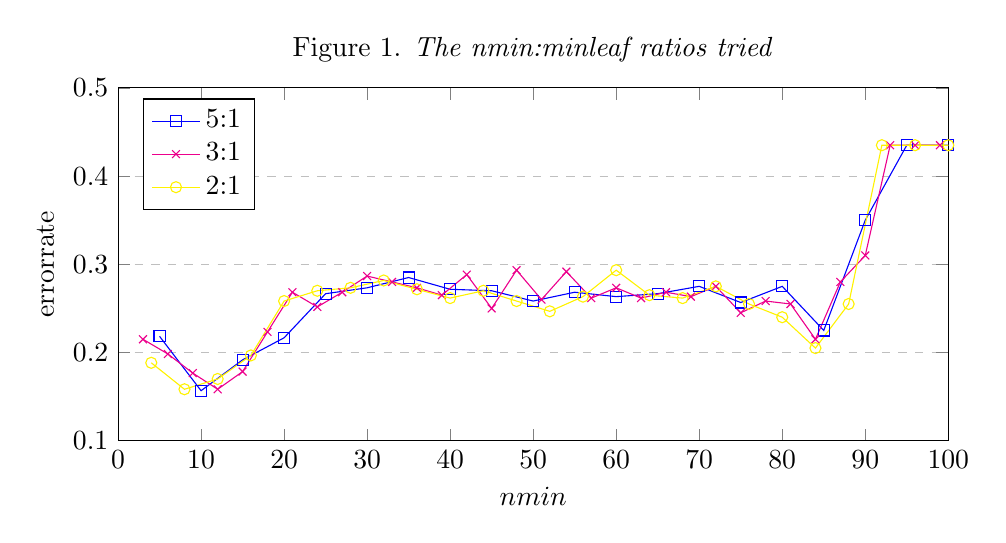
\begin{tikzpicture}
        \begin{axis}[
            title={Figure 1. \textit{The nmin:minleaf ratios tried}},
            xlabel={$nmin$},
            ylabel={errorrate},
            xmin=0, xmax=100,
            ymin=0.1, ymax=0.5,
            width=1\textwidth,
            height=0.5\textwidth,
            legend pos=north west,
            ymajorgrids=true,
            grid style=dashed
        ]
         
        \addplot[color=blue,mark=square,]
            coordinates {
                (5.0000000,0.2183333)(10.0000000,0.1566667)(15.0000000,0.1916667)(20.0000000,0.2166667)(25.0000000,0.2666667)(30.0000000,0.2733333)(35.000000,0.285000)(40.0000000,0.2716667)(45.000000,0.270000)(50.0000000,0.2583333)(55.0000000,0.2683333)(60.0000000,0.2633333)(65.0000000,0.2666667)(70.0000000,0.2750000)(75.0000000,0.2566667)(80.0000000,0.2750000)(85.0000000,0.2250000)(90.0000000,0.3500000)(95.0000000,0.4350000)(100.0000000,0.4350000)
            };
            \addlegendentry{5:1}
            
            \addplot[color=magenta,mark=x,]
                coordinates {
                    (3.000000,0.215000)(6.0000000,0.1983333)(9.0000000,0.1766667)(12.0000000,0.1583333)(15.0000000,0.1783333)(18.0000000,0.2233333)(21.0000000,0.2683333)(24.0000000,0.2516667)(27.0000000,0.2683333)(30.0000000,0.2866667)(33.000000,0.280000)(36.0000000,0.2733333)(39.000000,0.265000)(42.0000000,0.2883333)(45.000000,0.250000)(48.0000000,0.2933333)(51.0000000,0.2600000)(54.0000000,0.2916667)(57.0000000,0.2616667)(60.0000000,0.2733333)(63.0000000,0.2616667)(66.0000000,0.2683333)(69.0000000,0.2633333)(72.0000000,0.2750000)(75.0000000,0.2450000)(78.0000000,0.2583333)(81.0000000,0.2550000)(84.0000000,0.2150000)(87.0000000,0.2800000)(90.0000000,0.3100000)(93.00000,0.43500)(96.0000000,0.4350000)(99.0000000,0.4350000)
                };   
            \addlegendentry{3:1}

            \addplot[color=yellow,mark=o,]
                coordinates{
                    (4.0000000,0.1883333)(8.0000000,0.1583333)(12.000000,0.170000)(16.0000000,0.1966667)(20.0000000,0.2583333)(24.000000,0.270000)(28.0000000,0.2733333)(32.0000000,0.2816667)(36.0000000,0.2716667)(40.0000000,0.2616667)(44.0000000,0.2700000)(48.0000000,0.2583333)(52.0000000,0.2466667)(56.0000000,0.2633333)(60.0000000,0.2933333)(64.0000000,0.2650000)(68.0000000,0.2616667)(72.0000000,0.2750000)(76.0000000,0.2550000)(80.0000000,0.2400000)(84.0000000,0.2050000)(88.0000000,0.2550000)(92.0000000,0.4350000)(96.0000000,0.4350000)(100.0000000,0.4350000)
                };
            \addlegendentry{2:1}

        \end{axis}
    \end{tikzpicture}
    \\\\
    The results of performing another cross validation on all $nmin$ and $minleaf$ values where $nmin$ is between 8 and 20 with steps of 2 is shown in table 1. The values for $nmin$ 8, 18 and 20 have been omitted since they all scored well above an errorrate of $0.20$. The columns errorrate, nodes and leaves indicate the average of the 10 trees created during the cross validation.
    \\\\
    In table 1 the parameter pairs $(16,8),(16,4)$ and $(12,2)$ have the lowest errorrate, with $(16,8)$ also having a relatively small tree. Constructing a tree with these parameters on the trainingset, and predicting the classes of the testsample gives us the results as shown in table 2. The data in table 2 shows us that $nmin = 16$ and $minlead = 8$ are the best parameters, since they have the lowest errorrate and provide the smallest tree.

    \begin{table}[!htb]
    \small  

        \centering
        $\begin{array}{ *{6}{c} }
            \toprule
            nmin & minleaf & \text{errorrate} & \text{nodes} & \text{leaves} & \text{runtime(sec)} \\
            \midrule
                16 &  8  & 0.16  & 6.4 &  7.4 &  1.41 \\
                16 &  6  & 0.20  & 7.5 &  8.5 &  1.47 \\
                16 &  4  & 0.16  & 9.4 & 10.4 &  1.60 \\
                16 &  2  & 0.18  & 12.1 & 13.1 &  1.74 \\[1ex]
                14 &  7  & 0.21  & 7.8 &  8.8 &  1.50 \\
                14 &  5  & 0.15  & 8.9 &  9.9 &  1.57 \\
                14 &  3  & 0.19  & 11.6 & 12.6 &  1.79 \\
                14 &  1  & 0.24  & 17.2 & 18.2 &  1.96 \\[1ex]
                12 &  6  & 0.17  & 9.4 & 10.4 &  1.60 \\
                12 &  4  & 0.19 & 10.6 & 11.6 &  1.65 \\
                12 &  2  & 0.15 & 12.8 & 13.8 &  1.74 \\[1ex]
                10 &  5  & 0.17 & 10.8 & 11.8 &  1.66 \\
                10 &  3  & 0.18 & 12.4 & 13.4 &  1.72 \\
                10 &  1  & 0.22 & 18.4 & 19.4 &  1.96 \\
            \bottomrule
        \end{array}$
        \caption{\textit{Crossvalidation results.}}
    \end{table}

    \begin{table}[!htb]
    \small  

        \centering
        $\begin{array}{ *{5}{c} }
            \toprule
            nmin & minleaf & \text{errorrate} & \text{nodes} & \text{leaves} \\
            \midrule
                16 & 8 & 0.21 & 8 & 9 \\
                16 & 4 & 0.24 & 9 & 10 \\
                12 & 2 & 0.26 & 15 & 16 \\
            \bottomrule
        \end{array}$
        \caption{\textit{Trees grown on the complete trainingset.}}
    \end{table}

\clearpage
\section{Results}
The final tree, constructed with the parameters $nmin=16$ and $minleaf=8$ can be seen in figure 2. Splits are shown in the labels of edges. The numbers in the nodes mean the amount of instances labeled '0' and the amount of instances labeled '1' respectively. An obvious problem with this tree is the leaf with 6 zero-labeled instances and 11 one-labeled instances. The resubstitution error of this node is $1 - (11/17) \approx 0.35$, which is fairly high. A confusion matrix can be found in figure 2, the estimated errorrate is $0.21$.
\\\\
\tikzset{
  treenode/.style = {align=center, inner sep=0pt, text centered,
    font=\sffamily}
}

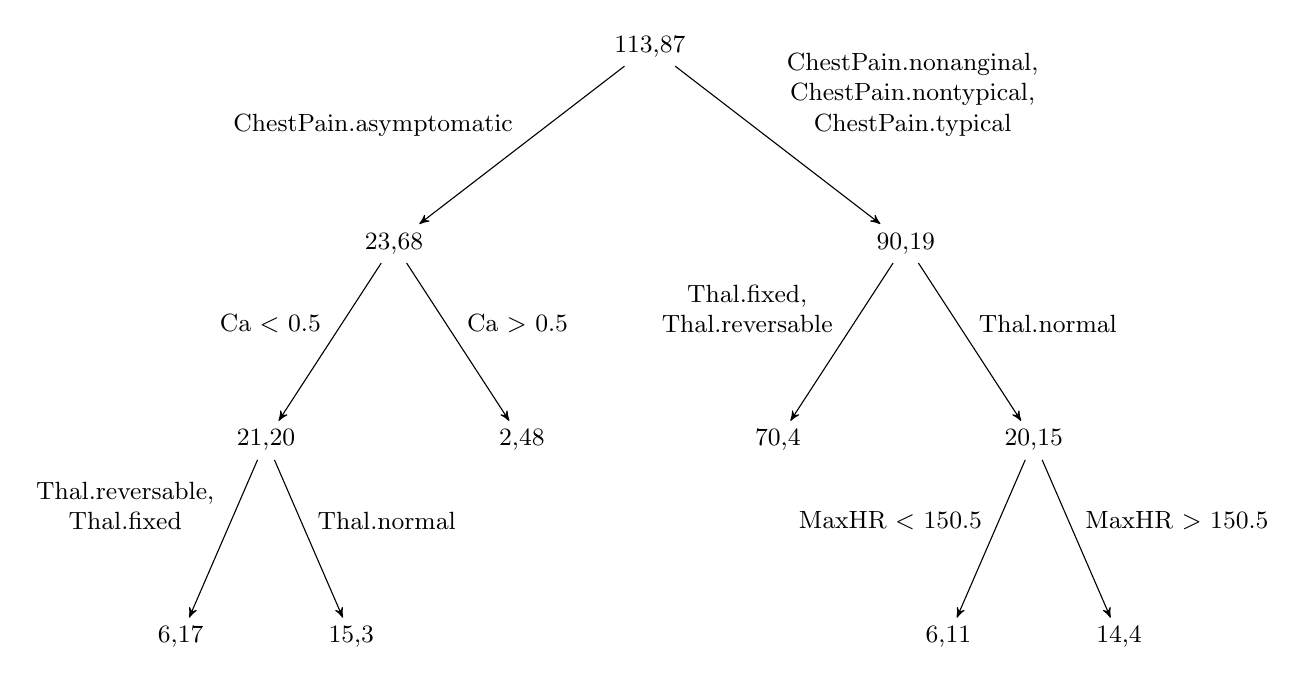
\begin{tikzpicture}[->,>=stealth',level/.style={sibling distance = 6.5cm/#1,
  level distance = 2.5cm}] 
  \small

\node {113,87} 
    child{ node {23,68} 
        child{ node {21,20}
                    child{ node {6,17}
                            edge from parent node[above left, align=center]{Thal.reversable, \\ Thal.fixed}
                    }
                    child{ node {15,3}
                            edge from parent node[above right]{Thal.normal}
                    }
                    edge from parent node[above left]{Ca $<$ 0.5}
        }
        child{ node {2,48} 
            edge from parent node[above right]{Ca $>$ 0.5}
        }
        edge from parent node[above left]{ChestPain.asymptomatic}
    }
    child { node{90,19}
        child{ node {70,4}
            edge from parent node[above left, align=center]{Thal.fixed, \\ Thal.reversable}
        }
        child{ node {20,15} 
            child{ node {6,11}
                edge from parent node[above left]{MaxHR $<$ 150.5}
            }
            child{ node {14,4}
                edge from parent node[above right]{MaxHR $>$ 150.5}
            }
            edge from parent node[above right]{Thal.normal}
        }
        edge from parent node[above right, align=center]{ChestPain.nonanginal, \\
                                            ChestPain.nontypical, \\ChestPain.typical}
    }                           
; 

\end{tikzpicture}

    \begin{table}[!htb]
        \centering
        $\begin{array}{c|cc}
            \toprule
                 & 0 & 1 \\
            \midrule
                0 & 42 & 16 \\
                1 & 5 & 34 \\
            \bottomrule
        \end{array}$
        \caption{\textit{Confusion matrix of the final tree.}}
    \end{table}

\end{document}